\documentclass{beamer}
\usepackage{ctex}  % comment this line to use pure English
\usepackage{minted}
\usepackage{caption}
\usepackage{subfigure}
% \usepackage{listings}
\usepackage[utf8]{inputenc}

% \setminted{xleftmargin=1cm}  % for code line number 

% \useoutertheme{split}
\usetheme{Madrid}
\usecolortheme{default}
\setbeamertemplate{navigation symbols}{}

\makeatother
\setbeamertemplate{footline}
{
  \leavevmode%
  \hbox{%
  \begin{beamercolorbox}[wd=.4\paperwidth,ht=2.25ex,dp=1ex,center]{author in head/foot}%
    \usebeamerfont{author in head/foot}\insertshortauthor
  \end{beamercolorbox}%
  \begin{beamercolorbox}[wd=.6\paperwidth,ht=2.25ex,dp=1ex,center]{title in head/foot}%
    \usebeamerfont{title in head/foot}\insertshorttitle\hspace*{3em}
    \insertframenumber{} / \inserttotalframenumber\hspace*{1ex}
  \end{beamercolorbox}}%
  \vskip0pt%
}
\makeatletter
\setbeamertemplate{navigation symbols}{}

%------------------------------------------------------------
%This block of code defines the information to appear in the
%Title page
\title[Parallel tricks in LLM] %optional
{Parallel tricks in LLM}

\subtitle{A quick view}

\author[Feng Wang] % (optional)
{Feng Wang\inst{1}}

\institute[baichuan] % (optional)
{
  \inst{1}%
  Baichuan\\
  wangfeng19950315@163.com
}

\date[beijing 2025] % (optional)
{Beijing, March 2025}

% \logo{\includegraphics[height=1cm]{overleaf-logo}}

\begin{document}

%The next statement creates the title page.
\frame{\titlepage}
%------------------------------------------------------------

%---------------------------------------------------------
%This block of code is for the table of contents after the title page
%---------------------------------------------------------

\begin{frame}
    \frametitle{Table of Contents}
    \tableofcontents
\end{frame}

% comment the following lines to add per-section table of contents
% -------------------------------------------
% \AtBeginSection[]
% {
%   \begin{frame}
%     \frametitle{Table of Contents}
%     \tableofcontents[currentsection]
%   \end{frame}
% }

%---------------------- Dist comm -------------------
\section{分布式通信原语}

\begin{frame}[fragile]
\frametitle{Broadcast \& Reduce}

\begin{figure}[h]
    \centering
    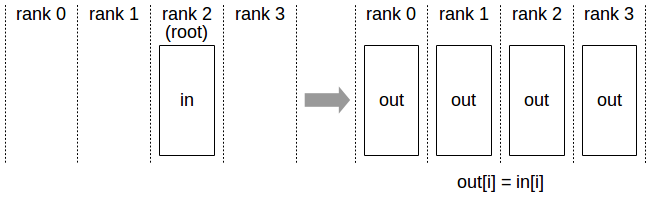
\includegraphics[width=0.8\textwidth]{broadcast.png}
    \captionsetup{labelformat=empty}
    \caption{broadcast}
\end{figure}

\begin{figure}[h]
    \centering
    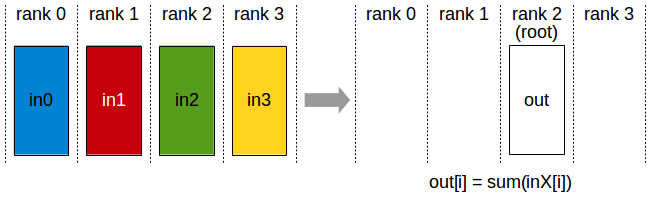
\includegraphics[width=0.8\textwidth]{reduce.png}
    \captionsetup{labelformat=empty}
    \caption{reduce}
\end{figure}


\end{frame}

\begin{frame}[fragile]
\frametitle{Scatter \& Gather}

\begin{figure}[h]
    \centering
    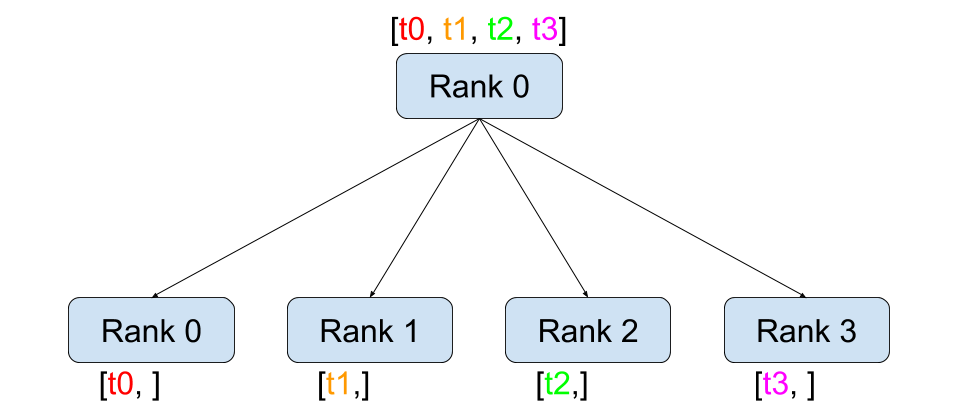
\includegraphics[height=0.3\textheight]{scatter.png}
    \captionsetup{labelformat=empty}
    \caption{scatter/one-to-all}
\end{figure}

\begin{figure}[h]
    \centering
    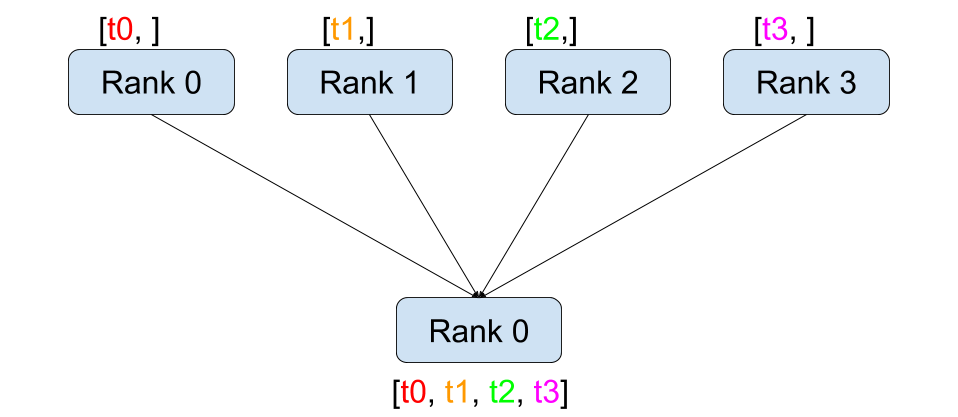
\includegraphics[height=0.3\textheight]{gather.png}
    \captionsetup{labelformat=empty}
    \caption{gather/all-to-one}
\end{figure}

\end{frame}


\begin{frame}[fragile]
\frametitle{Reduce-Scatter \& All-Gather}

\begin{figure}[h]
    \centering
    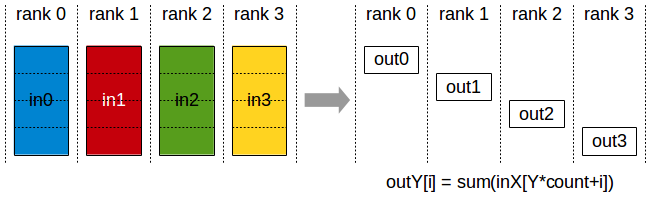
\includegraphics[width=0.8\textwidth]{reducescatter.png}
    \captionsetup{labelformat=empty}
    \caption{reduce-scatter = reduce + scatter}
\end{figure}

\begin{figure}[h]
    \centering
    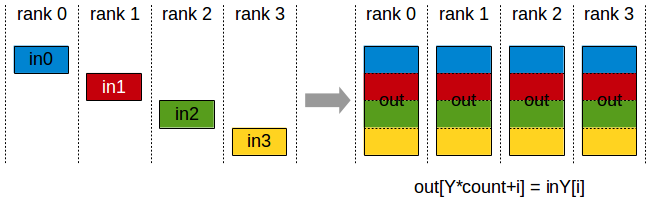
\includegraphics[width=0.8\textwidth]{allgather.png}
    \captionsetup{labelformat=empty}
    \caption{all-gather = gather + broadcast}
\end{figure}

\end{frame}


\begin{frame}[fragile]
\frametitle{All-Reduce \& All-to-All}

\begin{figure}[h]
    \centering
    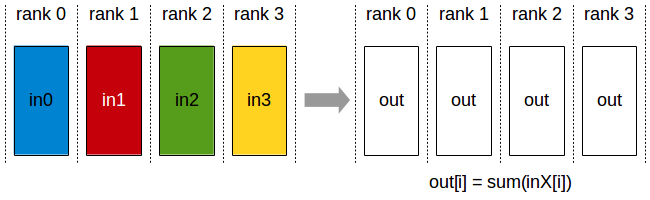
\includegraphics[height=0.3\textheight]{allreduce.png}
    \captionsetup{labelformat=empty}
    \caption{all-reduce = reduce + broadcast = reduce-scatter + all-gather}
\end{figure}

\begin{figure}[h]
    \centering
    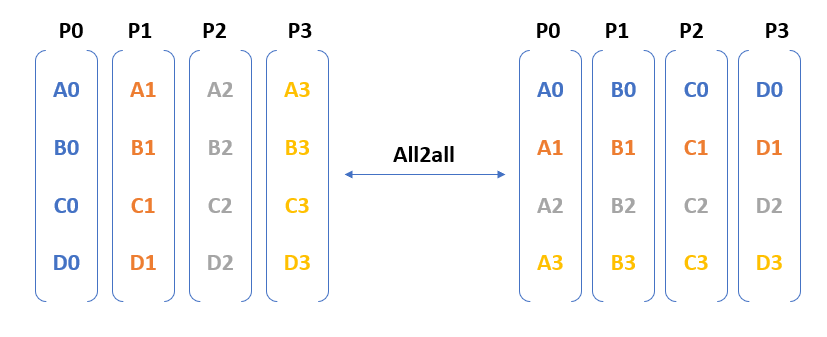
\includegraphics[height=0.35\textheight]{all2all.png}
    \captionsetup{labelformat=empty}
    \caption{all-to-all / transpose}
\end{figure}

\end{frame}


\begin{frame}[fragile]
\frametitle{Barrier}

\begin{figure}[h]
    \centering
    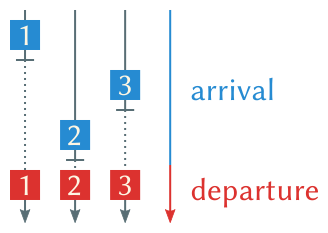
\includegraphics[height=0.3\textheight]{barrier.png}
    \captionsetup{labelformat=empty}
    \caption{barrier}
\end{figure}

\begin{figure}[h]
    \centering
    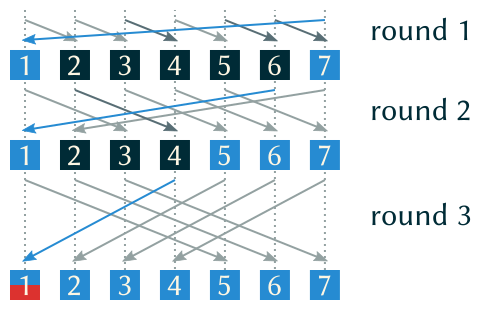
\includegraphics[height=0.35\textheight]{dissemination.png}
    \captionsetup{labelformat=empty}
    \caption{dissemination barrier}
\end{figure}

\end{frame}

\begin{frame}[fragile]
\frametitle{Quick test}

做一些简单的随堂测试:

\begin{itemize}
    \item<1-> all-to-all的inverse 操作是什么?\newline
    inverse语意:求函数f,使得下面恒为True
    \begin{minted}{python}
    f(all2all(x)) == x
    \end{minted}

    \item<2-> 对于一个大小为n的参数,做ring-all-reduce操作,需要多少通信量?\newline

    \item<3-> tree-all-reduce和ring-all-reduce谁更快?两个算法计算的结果一样吗?\newline

\end{itemize}
\end{frame}

%---------------------- Parallel Tricks ----------------

\section{Parallel tricks}

\begin{frame}[fragile]
\frametitle{Data Parallel}
\begin{figure}[h]
    \centering
    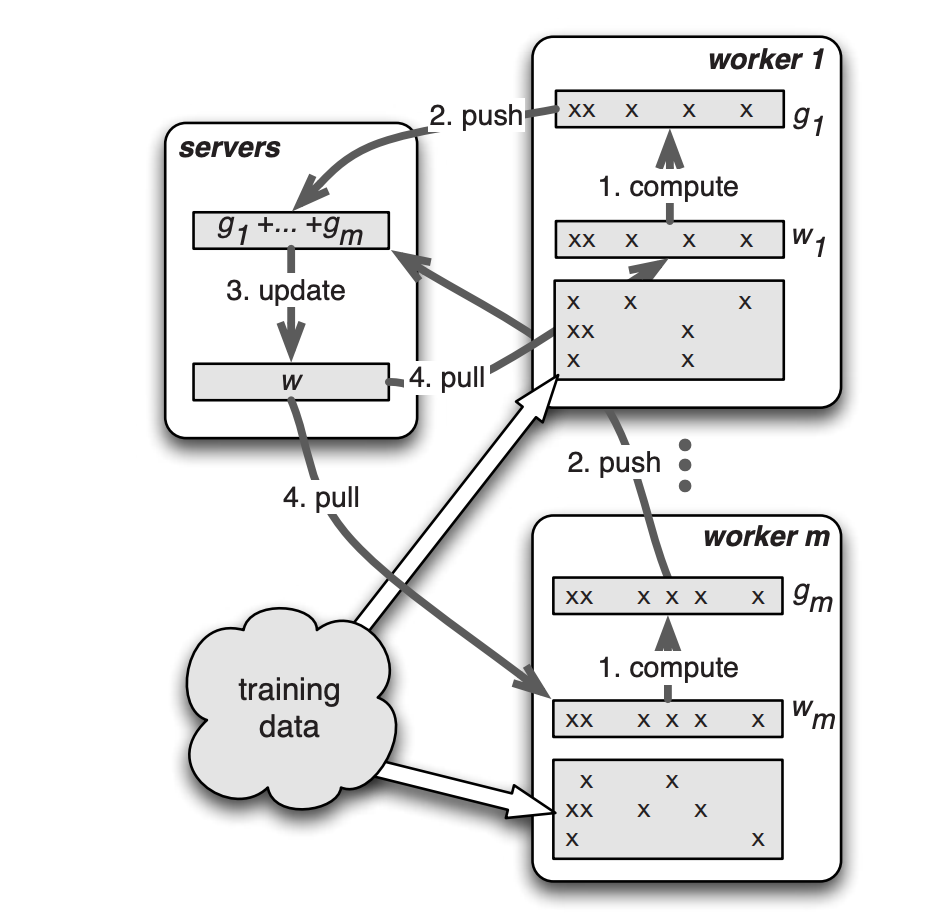
\includegraphics[width=0.35\textwidth]{parameter_server.png}
    \hfill
    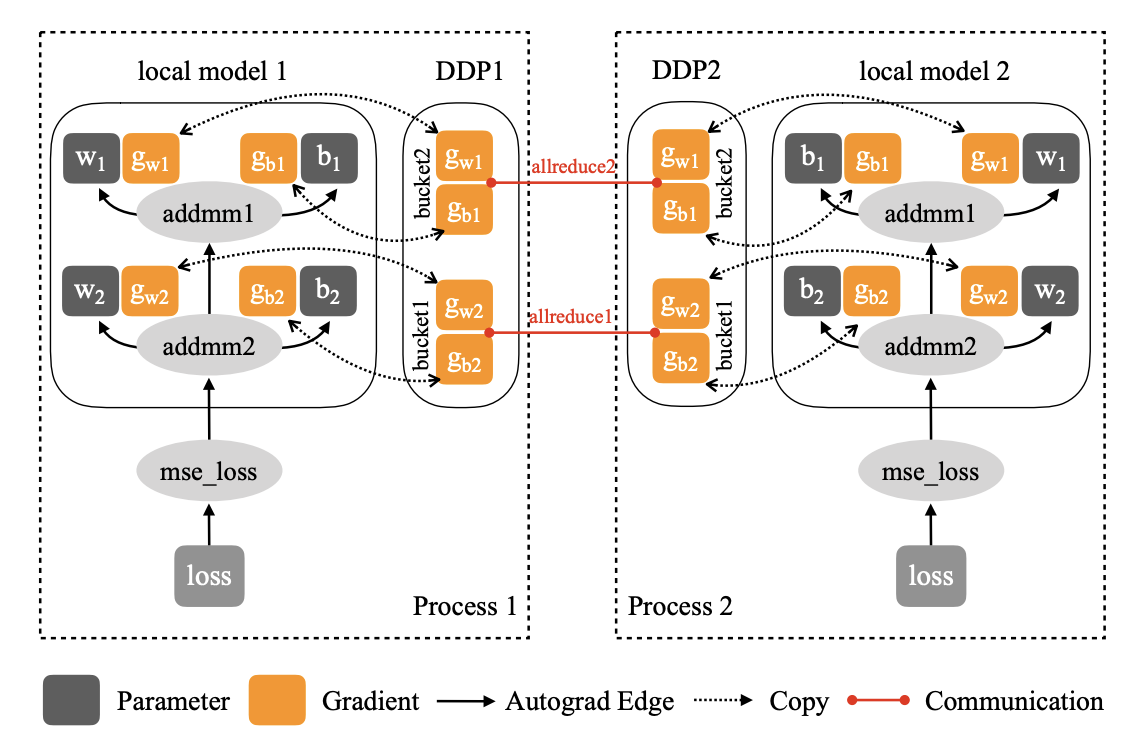
\includegraphics[width=0.6\textwidth,height=0.5\textheight]{torch_ddp.png}
    \captionsetup{labelformat=empty}
    \caption{Parameter Server(left) vs Torch DDP(right)}
\end{figure}

Parameter Server: 一个中心节点负责\textcolor{red}{gather},参数更新和\textcolor{red}{broadcast},worker节点负责计算梯度\newline
Torch DDP: 每个worker节点都有一份完整的模型,计算梯度后做\textcolor{red}{all-reduce},然后更新参数

\end{frame}

\begin{frame}[fragile]
\frametitle{Pipeline Parallel}

\begin{figure}[h]
    \centering
    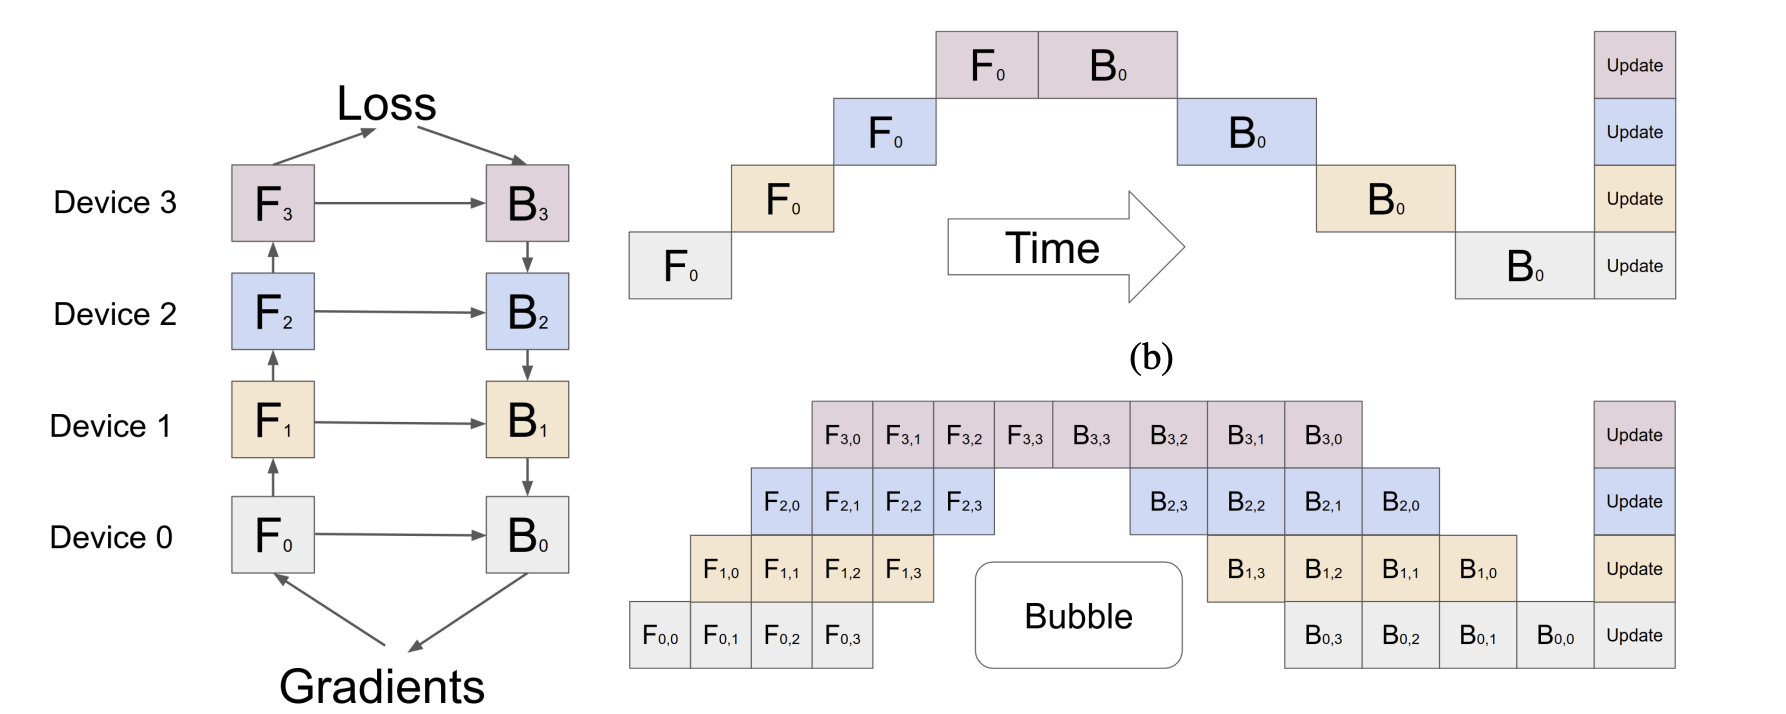
\includegraphics[width=0.8\textwidth]{gpipe.png}
    \captionsetup{labelformat=empty}
    \caption{GPipe}

\end{figure}

Pipeline Parallel: 将模型切分成多个stage,每个stage计算一部分,然后将结果传递给下一个stage。\newline
相比Tensor Parallel,PP的通信量更小(只在某一个阶段传送激活值)\newline
缺点在于会有bubble,实现复杂度高,且对于模型结构有一定要求(对residual、transformer的hidden states不友好)。

\end{frame}

\begin{frame}[fragile]
\frametitle{Tensor Parallel}

\begin{figure}[h]
    \centering
    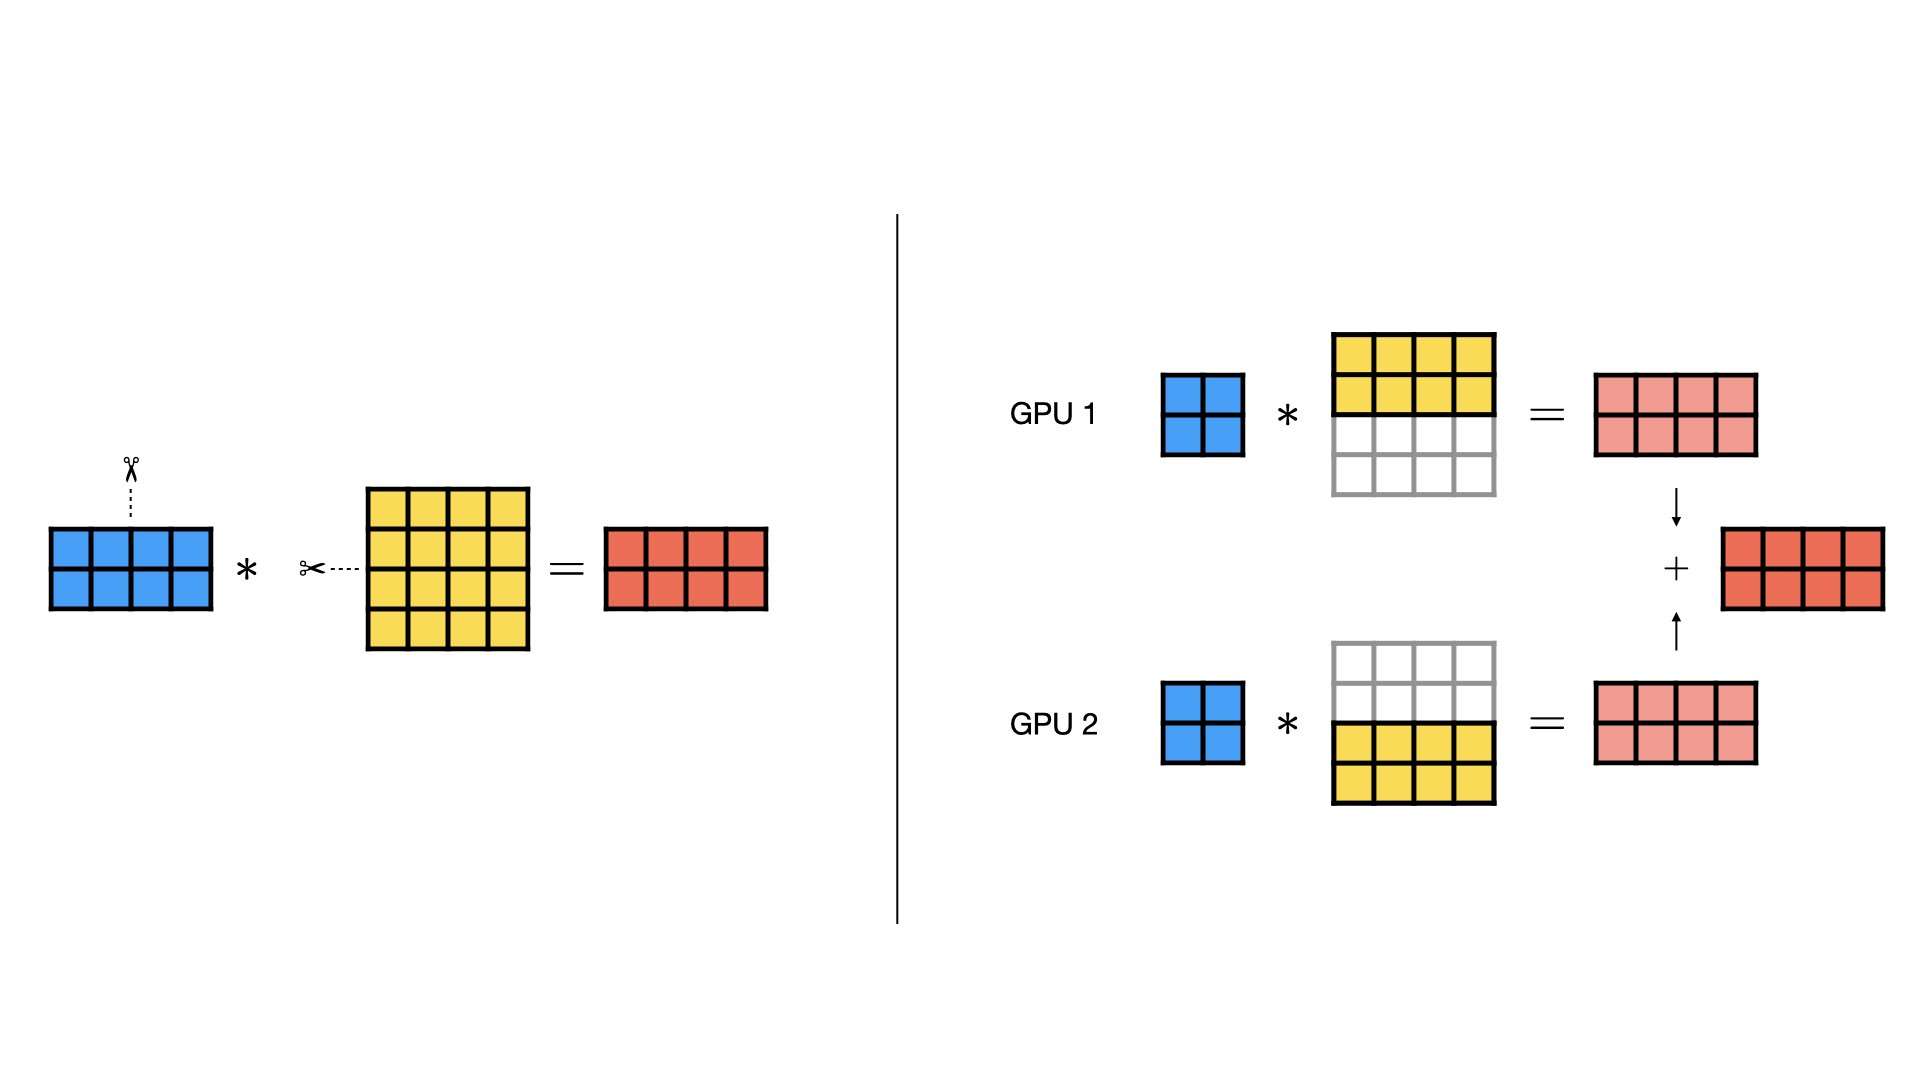
\includegraphics[width=0.7\textwidth]{tp-rowwise.jpeg}
    \captionsetup{labelformat=empty}
    \caption{Row Tensor Parallel}
\end{figure}

Row TP: 将weights沿着row切分,forward做\textcolor{red}{all-reduce},backward做\textcolor{red}{all-gather}\newline
\end{frame}


\begin{frame}[fragile]
\frametitle{Tensor Parallel}

\begin{figure}[h]
    \centering
    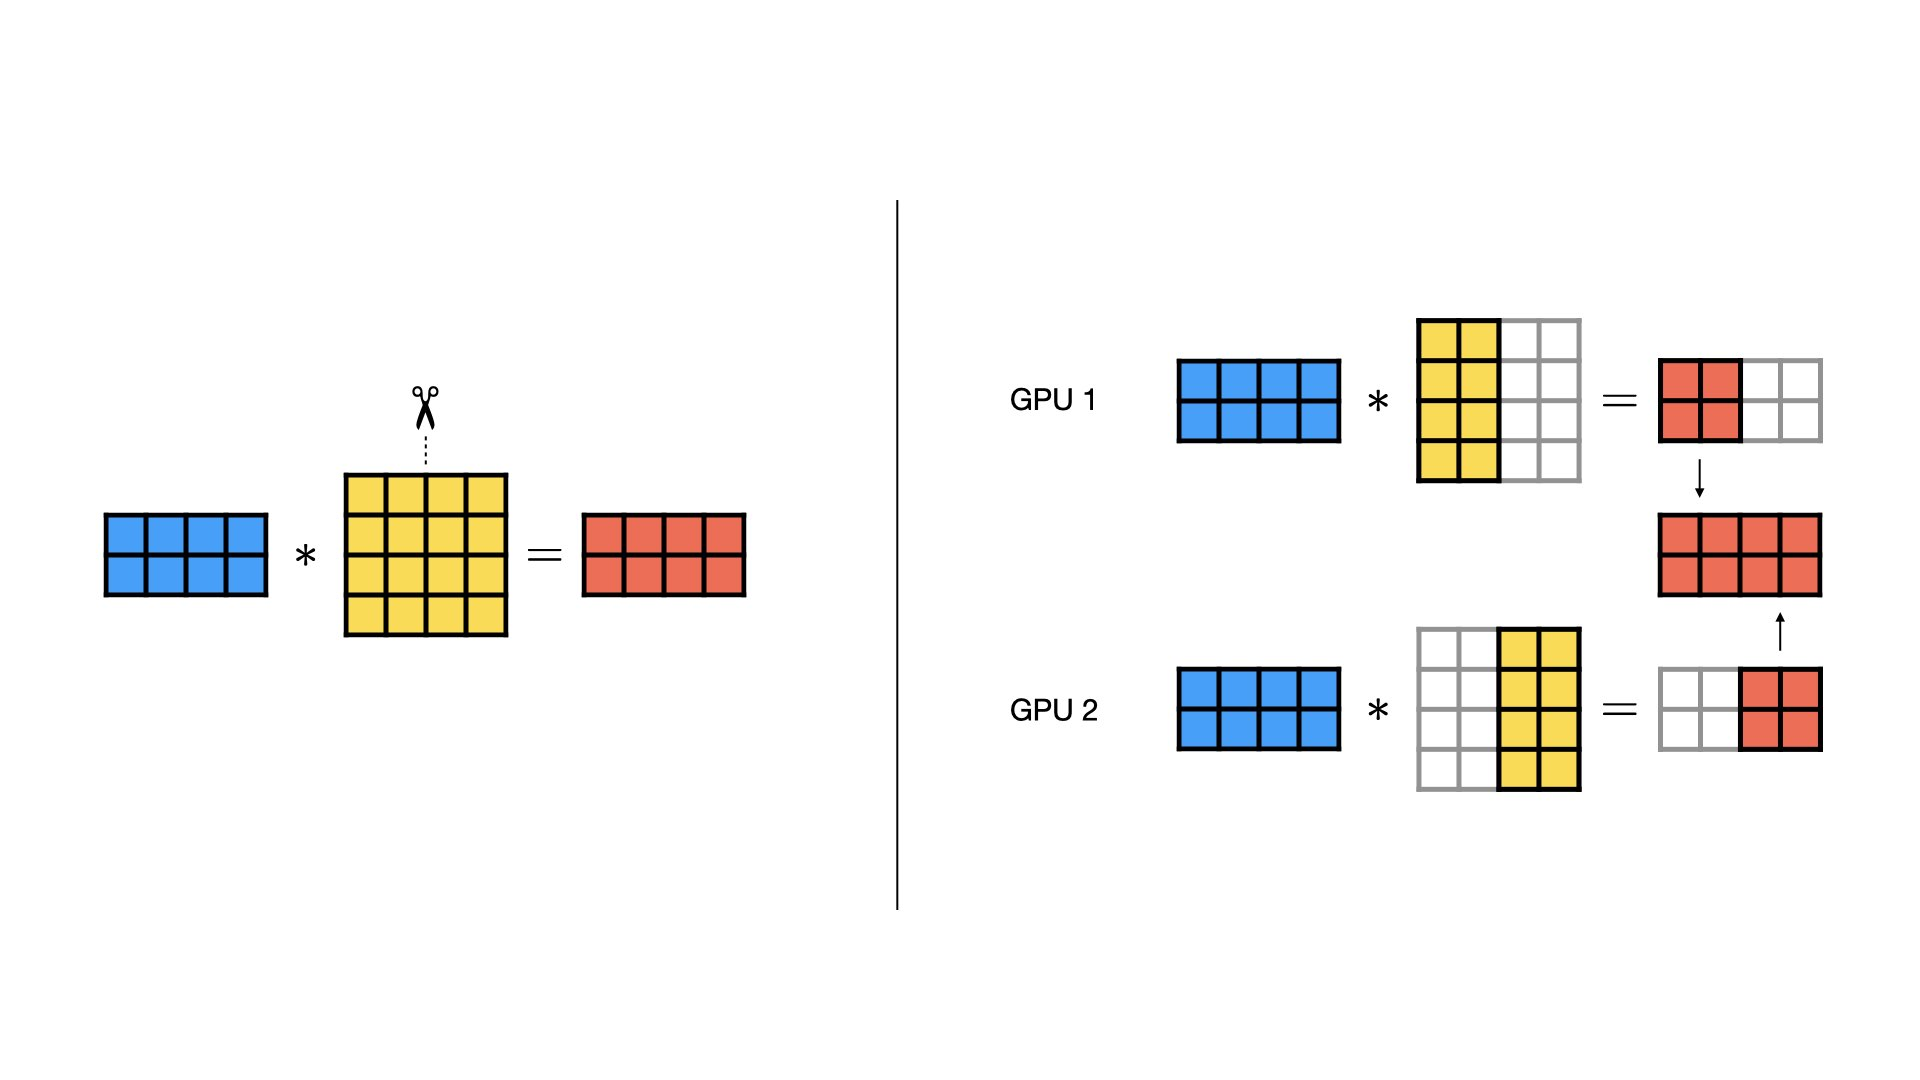
\includegraphics[width=0.7\textwidth]{tp-colwise.jpeg}
    \captionsetup{labelformat=empty}
    \caption{Column Tensor Parallel}
\end{figure}

Col TP: 将weights沿着column切分,forward做\textcolor{red}{all-gather},backward做\textcolor{red}{all-reduce}(和Row相反)\newline

\end{frame}


\begin{frame}[fragile]
\frametitle{Tensor Parallel}

\begin{figure}[h]
    \centering
    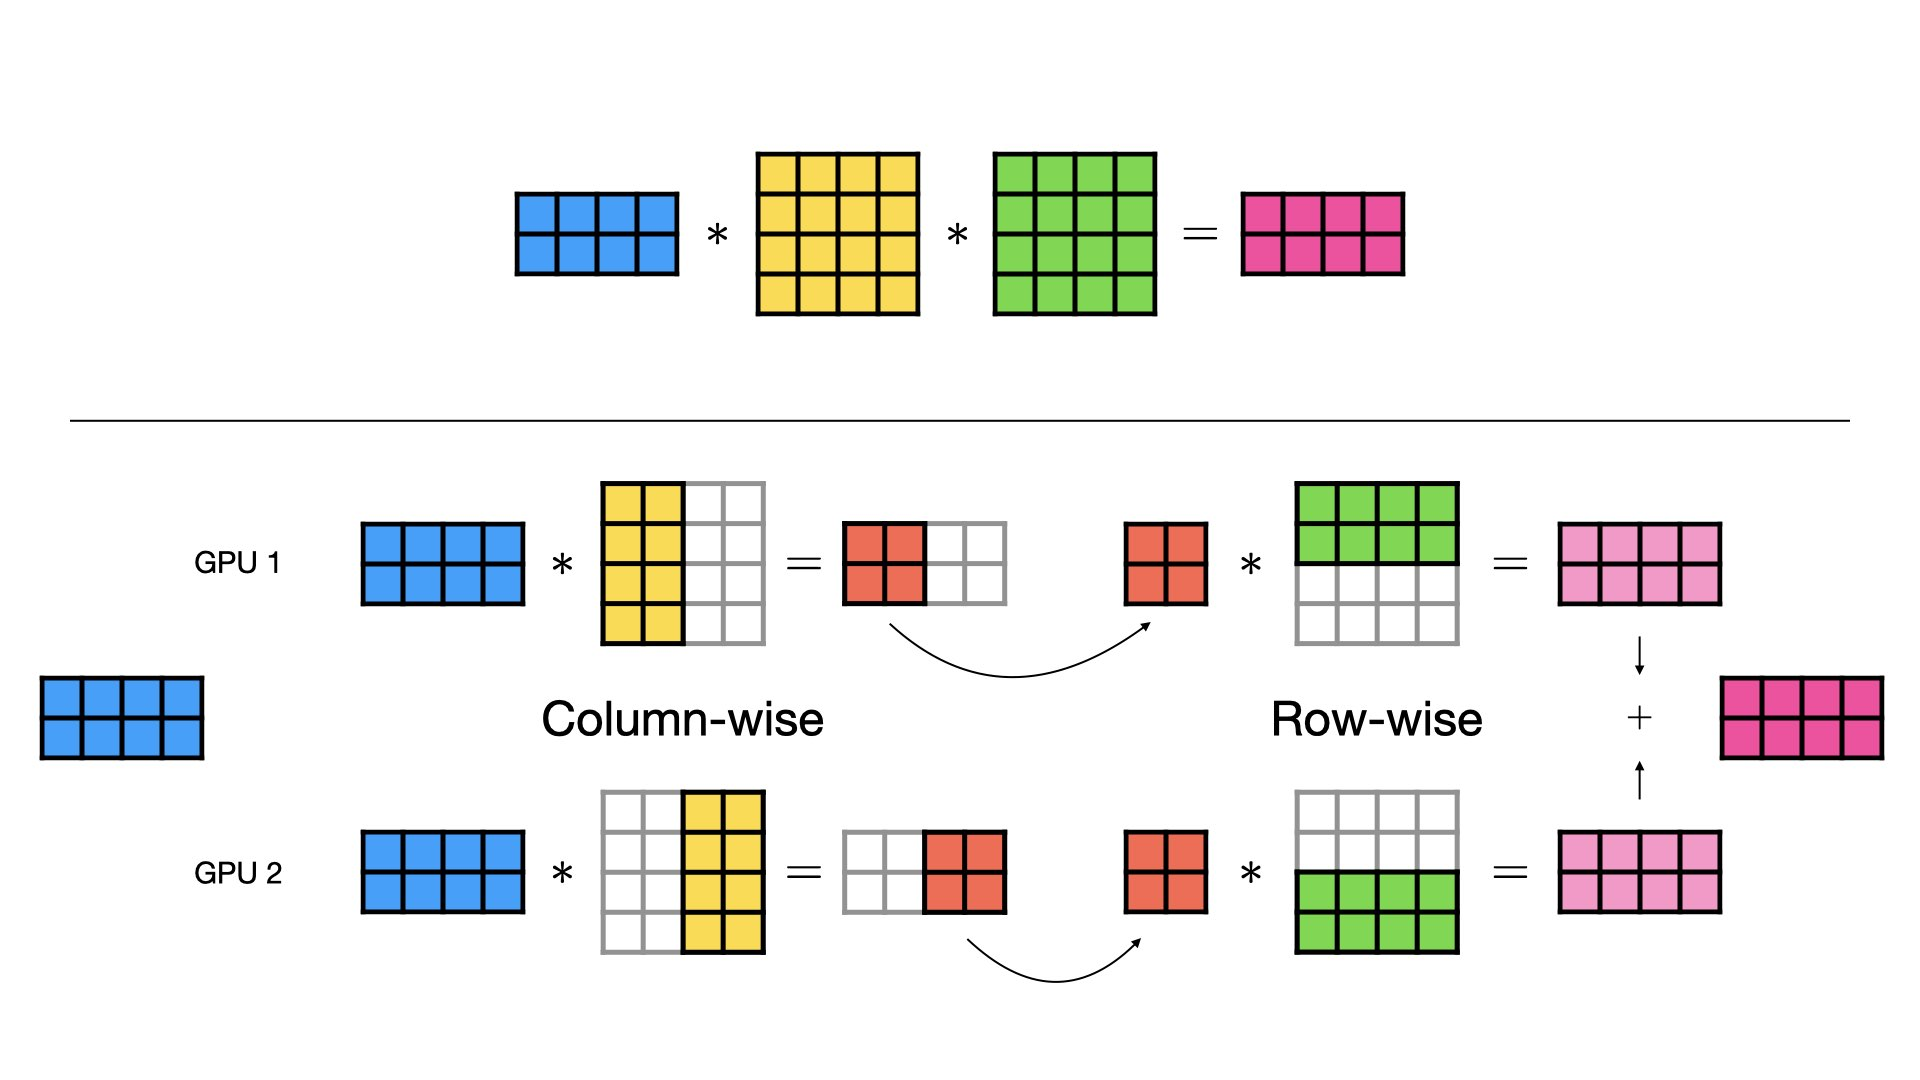
\includegraphics[width=0.7\textwidth]{tp-combined.jpeg}
    \captionsetup{labelformat=empty}
    \caption{Combined Tensor Parallel}
\end{figure}
Hybrid TP: 先Col TP,然后Row TP,forward的时候 Col TP不做all-gather

\end{frame}


\begin{frame}[fragile]
\frametitle{Sequence Parallel (Megatron-LM)}

\begin{figure}[h]
    \centering
    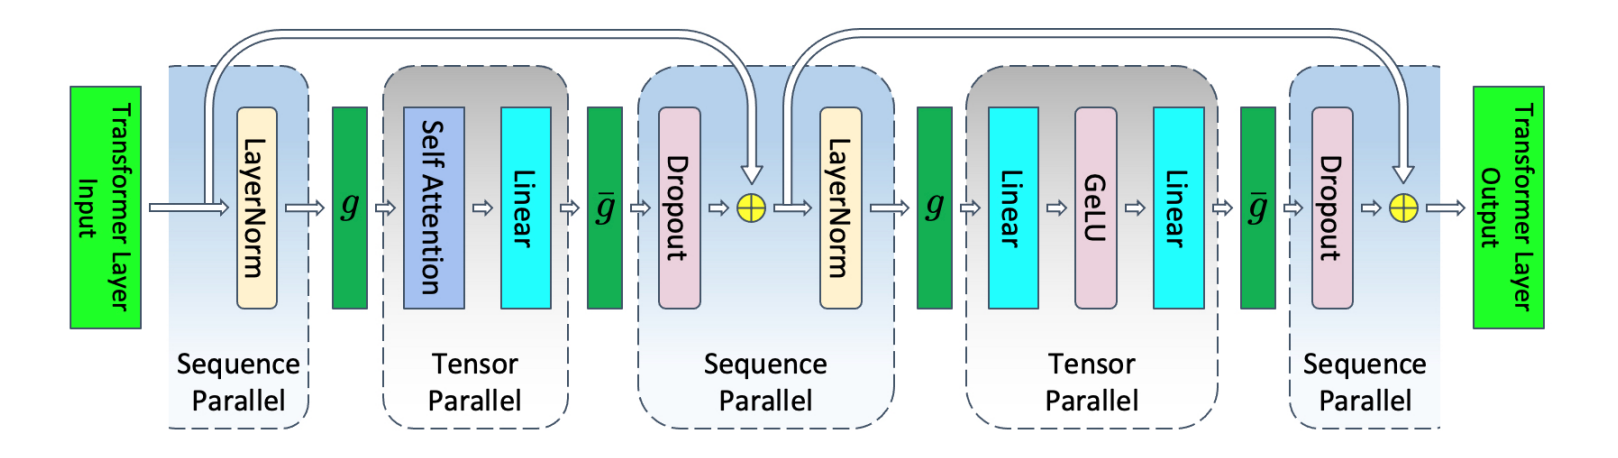
\includegraphics[width=0.8\textwidth]{megatron_sp.png}
    \captionsetup{labelformat=empty}
    \caption{Megatron SP}
\end{figure}

Megatron-LM的Sequence Parallel是将hidden states沿着sequence dim切分,layernorm本身被切开(因为只apply最后一个dim)\newline
MHSA部分做TP:q/k/v做Col TP,output做Row TP\newline
g function:\textcolor{red}{all-gather}\newline
$\bar{g}$ function:\textcolor{red}{reduce-scatter}

\end{frame}


\begin{frame}[fragile]
\frametitle{Sequence Parallel (Megatron-LM)}

\begin{figure}[h]
    \centering
    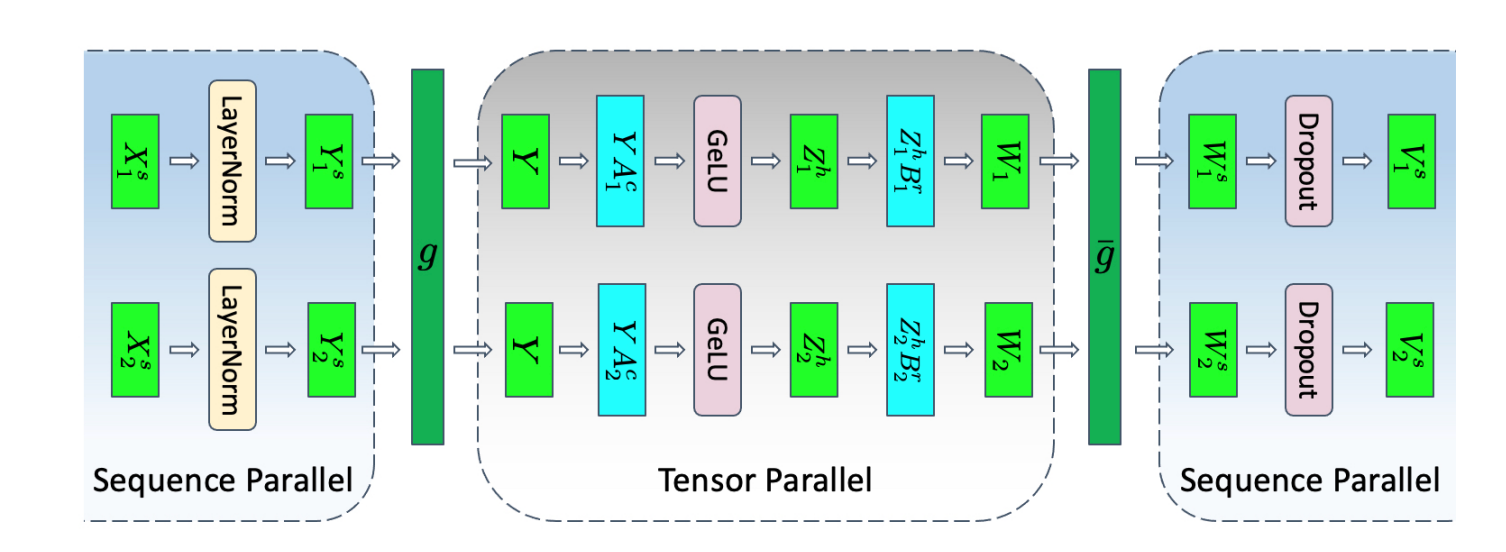
\includegraphics[width=0.8\textwidth]{megatron_sp_inside.png}
    \captionsetup{labelformat=empty}
    \caption{inside Megatron SP}
\end{figure}

Megatron-LM的Sequence Parallel是将hidden states沿着sequence dim切分,layernorm本身被切开(因为只apply最后一个dim)\newline
MHSA部分做TP:q/k/v做Col TP,output做Row TP\newline
g function:\textcolor{red}{all-gather}\newline
$\bar{g}$ function:\textcolor{red}{reduce-scatter}

\end{frame}


\begin{frame}[fragile]
\frametitle{Sequence Parallel (Deepspeed-Ulysses)}

\begin{figure}[h]
    \centering
    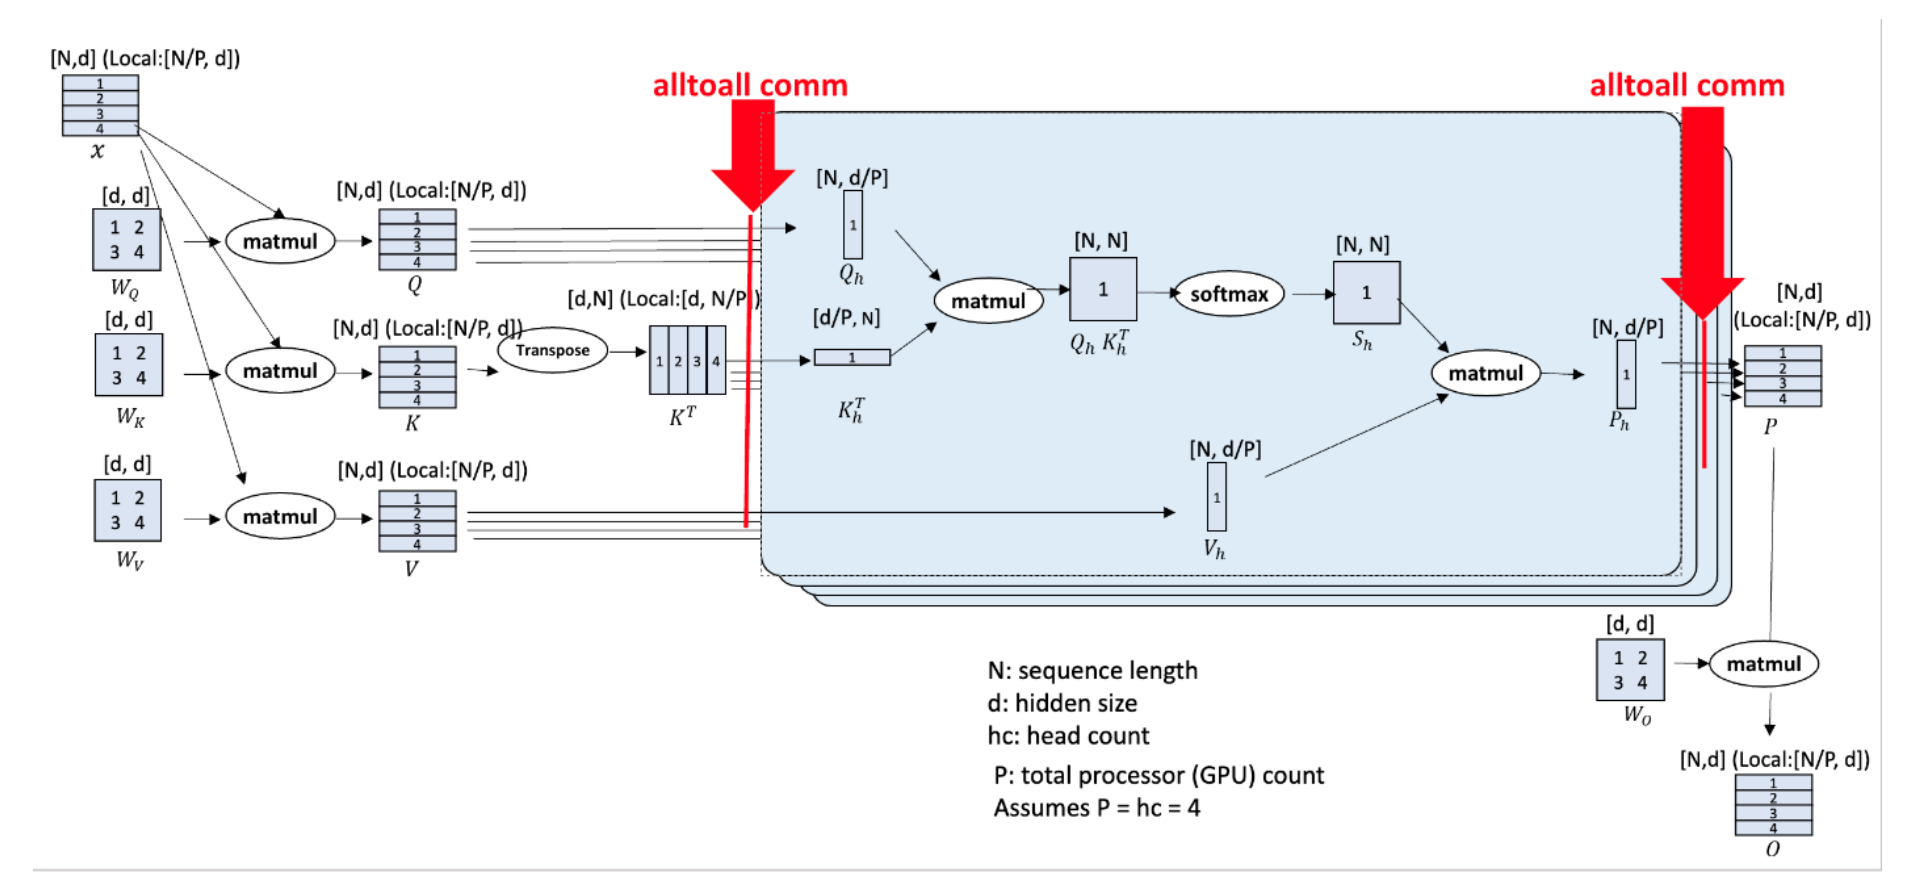
\includegraphics[width=0.8\textwidth]{ds_ulysess.png}
    \captionsetup{labelformat=empty}
    \caption{Deepspeed SP}
\end{figure}

deepspeed sp的做法很简单,将hidden states沿着sequence dim切分,然后对q/k/v做\textcolor{red}{all-to-all},正常计算attention,最后对output做\textcolor{red}{all-to-all}\newline
q/k/v的all-to-all是沿着head dim做切分,沿着sequence dim做拼接\newline
output的all-to-all是沿着seqence dim做切分,沿着head dim做拼接\newline

\end{frame}


\begin{frame}[fragile]
\frametitle{Sequence Parallel (Deepspeed-Ulysses)}

代码实现
\begin{minted}{python}
q = linear_transform(x, self.q_proj)
k = linear_transform(x, self.k_proj)
v = linear_transform(x, self.v_proj)

h = self.num_heads
q,k,v = split_heads(q, h), split_heads(k, h), split_heads(v, h)

q = all_to_all_array(q, split_axis=1, concat_axis=-2)
k = all_to_all_array(k, split_axis=1, concat_axis=-2)
v = all_to_all_array(v, split_axis=1, concat_axis=-2)

out = self.attn(q, k, v, mask=mask)
out = all_to_all_array(out, split_axis=-2, concat_axis=1)

out = np.swapaxes(out, 1, 2).reshape(batch, -1, dim)
return linear_transform(out, self.out_proj)
\end{minted}

\end{frame}

\begin{frame}[fragile]
\frametitle{Sequence Parallel (Deepspeed-Ulysses)}

DeepSpeed SP的优点\newline
1. 通信量小(\textcolor{red}{4Nd/P},P为device数),实现简单,对模型结构要求低。\newline
2. 不侵入attention实现,可以和flash attn正交使用\newline
3. 在在序列长度N非常大时,增加卡数可以降低通信量,如果N和P都是线性增长,单卡的通讯量不会变化\newline
4. DeepSpeed主推,和ZeRO3结合使用,进一步节省显存\newline\newline

缺点\newline
1. 并行度不会超过head的数量,对于head数量少的模型,可能会有性能瓶颈(比如1M窗口长的0.5B模型)\newline
2. 对底层通信硬件拓扑结构要求高\newline

\end{frame}


\begin{frame}[fragile]
\frametitle{Maybe Next Time}

1. Context Parallel\newline
需要前置讲解flash attn,ring attn\newline
涉及到load balance的问题,还在学习中\newline

2. Expert Parallel\newline
EP的想法很简单,每台机器都包含部分专家\newline
EP的实现稍稍有点复杂,还在学习中\newline

\end{frame}


%---------------------- ZeRO ----------------

\section{ZeRO}

\begin{frame}[fragile]
\frametitle{ZeRO overview}

\begin{figure}[h]
    \centering
    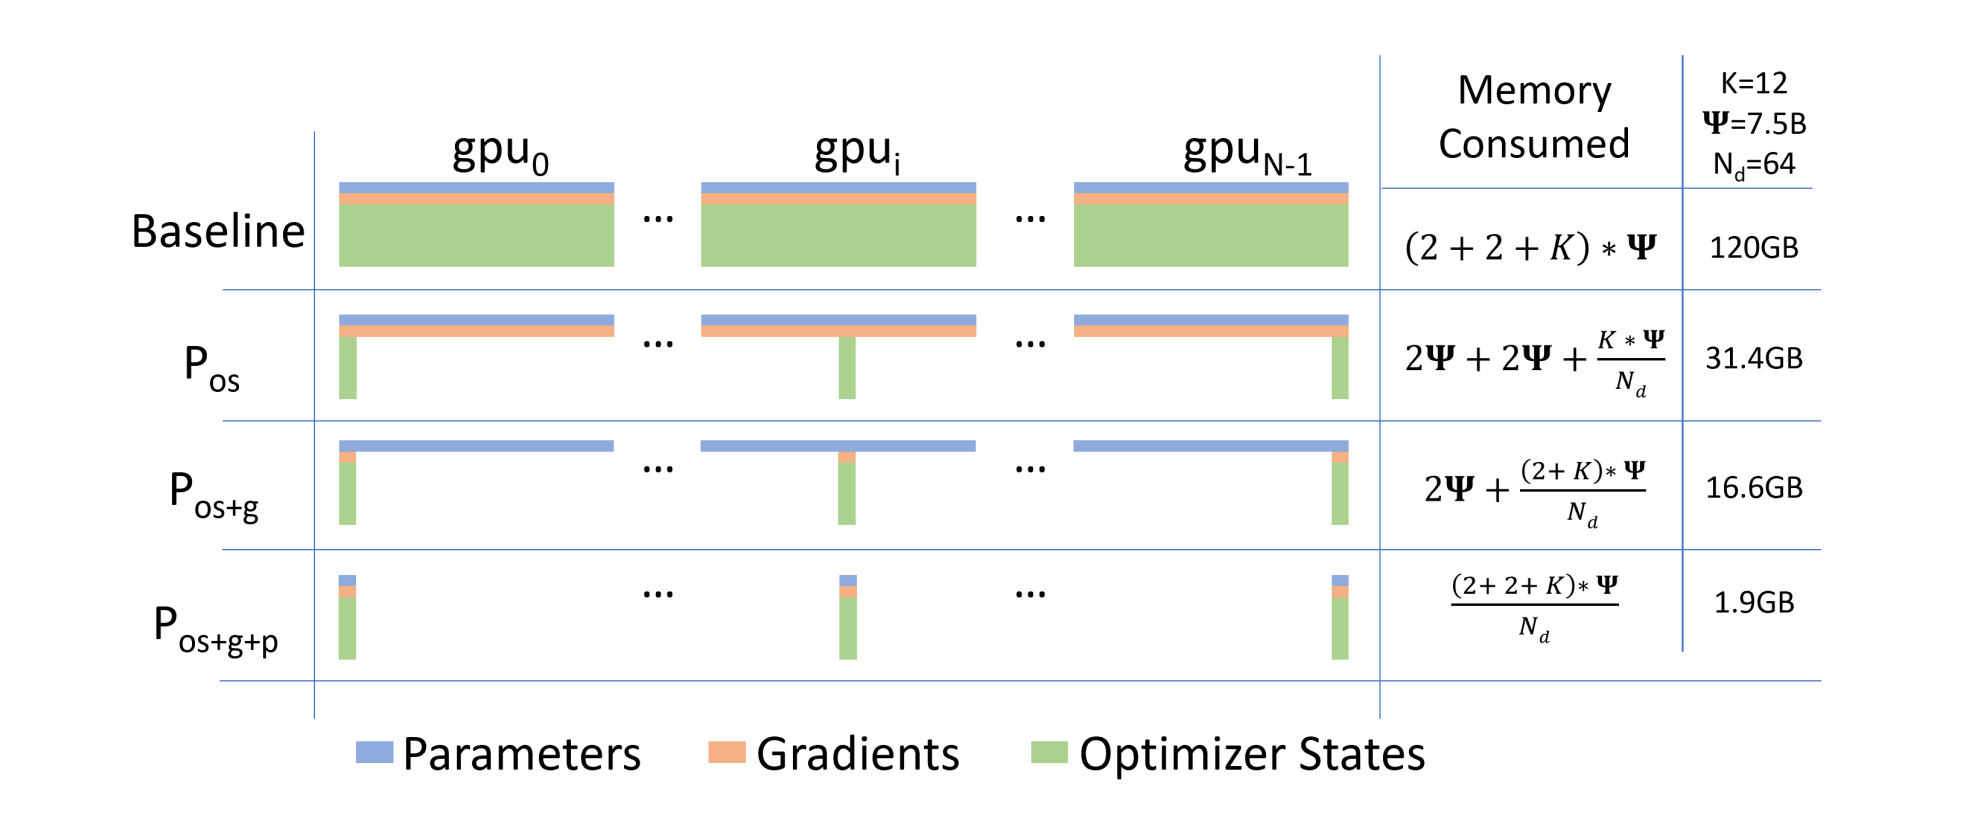
\includegraphics[width=0.8\textwidth]{zero.png}
    \captionsetup{labelformat=empty}
    \caption{ZeRO 1/2/3对比}
\end{figure}

ZeRO 1: 仅仅将optimizer state切分\newline
ZeRO 2: 将optimizer state,gradient切分\newline
ZeRO 3: 将optimizer state,gradient,parameter都切分\newline

\end{frame}


\begin{frame}[fragile]
\frametitle{Process}

ZeRO1: forward/backward正常,step阶段,对grad做\textcolor{red}{all-reduce},仅计算有state的grad计算param delta,更新参数后做all-gather\newline
通信量 \(2\phi + 1\phi = 3\phi\)\newline\newline

ZeRO2: forward/backward正常,step阶段,对grad做\textcolor{red}{reduce-scatter}(因为梯度已经被切分了),更新参数后做all-gather\newline
通信量 \(1\phi + 1\phi = 2\phi\)\newline\newline

ZeRO3: init阶段做broadcast然后切分(等价scatter),forward阶段做\textcolor{red}{all-gather}(收集全部正确的params)\textcolor{red}{然后释放},
backward做\textcolor{red}{all-gather}然后释放,step阶段做\textcolor{red}{reduce-scatter}\newline
通信量 \(1\phi + 1\phi + 1\phi = 3\phi\)\newline

\end{frame}

%---------------------- Ref ----------------

\section{Reference}

\begin{frame}[fragile]
\frametitle{参考链接}

引用来源:\newline
\href{https://docs.nvidia.com/deeplearning/nccl/user-guide/docs/usage/collectives.html}{\color{blue}[1] NCCL collectives}\newline
\href{https://pytorch.org/tutorials/intermediate/dist_tuto.html#communication-backends}{\color{blue}[2] PyTorch comm}\newline
\href{https://www.usenix.org/system/files/conference/osdi14/osdi14-paper-li_mu.pdf}{\color{blue}[3] Parameter Server}\newline
\href{https://arxiv.org/pdf/2006.15704}{\color{blue}[4] Pytroch distributed}\newline
\href{https://arxiv.org/pdf/1811.06965}{\color{blue}[5] GPipe}\newline
\href{https://lightning.ai/docs/fabric/2.4.0/advanced/model_parallel/tp.html}{\color{blue}[6] Tensor Parallel doc}\newline
\href{https://arxiv.org/pdf/2205.05198}{\color{blue}[7] Megatron SP paper}\newline
\href{https://arxiv.org/pdf/2309.14509}{\color{blue}[8] Deepspeed Ulysses paper}\newline
\href{https://github.com/deepspeedai/DeepSpeed/blob/master/deepspeed/runtime/zero/stage_1_and_2.py}{\color{blue}[9] ZeRO stage 1/2实现}\newline
\href{https://github.com/deepspeedai/DeepSpeed/blob/master/deepspeed/runtime/zero/stage3.py}{\color{blue}[10] ZeRO stage 3实现}\newline

\end{frame}


\end{document}
